% !TeX spellcheck = en_US
% !TeX encoding = utf8
% !TeX program = xelatex
% !BIB program = bibtex
% \documentclass[mathserif,compress,12pt]{ctexbeamer}
\documentclass[12pt,notes,mathserif]{beamer}
% \documentclass[draft]{beamer}	
\usetheme{Singapore}
% \usetheme{Hannover}
%\usepackage{pgfpages}
%\setbeameroption{show notes on second screen}

\usepackage[british]{babel}
\usepackage{graphicx,hyperref,url}
% \usepackage{ru}
\usepackage{mmstyles}

\usepackage{listings}
\usefonttheme[onlymath]{serif}
\usepackage{fontspec}
\usepackage{xeCJK}
% \pgfdeclareimage[width=\paperwidth,height=\paperheight]{bg}{background}
% \setbeamertemplate{background}{\pgfuseimage{bg}}
%% columns
\newcommand{\begincols}[1]{\begin{columns}{#1}}
\newcommand{\stopcols}{\end{columns}}
% \usepackage[backend=biber]{biblatex}
% \bibliography{./ref.bib}
%\addbibresource{ref.bib}
\usepackage{indentfirst}
\usepackage{longtable}
\usepackage{float}
%\usepackage{picins}
\usepackage{rotating}
\usepackage{subfigure}
\usepackage{tabu}
\usepackage{amsmath}
\usepackage{amssymb}
\usepackage{setspace}
\usepackage{amsfonts}
\usepackage{appendix}
\usepackage{listings}
\usepackage{xcolor}
\usepackage{colortbl}
\usepackage{geometry}
% \setCJKfamilyfont{cjkhwxk}{SimSun}
% \newcommand*{\cjkhwxk}{\CJKfamily{cjkhwxk}}
%\newfontfamily{\consolas}{Consolas}
%\newfontfamily{\monaco}{Monaco}
%\setmonofont[Mapping={}]{Consolas}	%英文引号之类的正常显示,相当于设置英文字体
%\setsansfont{Consolas} %设置英文字体 Monaco, Consolas,  Fantasque Sans Mono
% \setmainfont{Times New Roman}
% \newfontfamily{\consolas}{Times New Roman}
% \newfontfamily{\monaco}{Arial}
% \setCJKmainfont{Times New Roman}
%\setmainfont{MONACO.TTF}
%\setsansfont{MONACO.TTF}
\newcommand{\verylarge}{\fontsize{60pt}{\baselineskip}\selectfont}  
\newcommand{\chuhao}{\fontsize{44.9pt}{\baselineskip}\selectfont}  
\newcommand{\xiaochu}{\fontsize{38.5pt}{\baselineskip}\selectfont}  
\newcommand{\yihao}{\fontsize{27.8pt}{\baselineskip}\selectfont}  
\newcommand{\xiaoyi}{\fontsize{25.7pt}{\baselineskip}\selectfont}  
\newcommand{\erhao}{\fontsize{23.5pt}{\baselineskip}\selectfont}  
\newcommand{\xiaoerhao}{\fontsize{19.3pt}{\baselineskip}\selectfont} 
\newcommand{\sihao}{\fontsize{14pt}{\baselineskip}\selectfont}      % 字号设置  
\newcommand{\xiaosihao}{\fontsize{12pt}{\baselineskip}\selectfont}  % 字号设置  
\newcommand{\wuhao}{\fontsize{10.5pt}{\baselineskip}\selectfont}    % 字号设置  
\newcommand{\xiaowuhao}{\fontsize{9pt}{\baselineskip}\selectfont}   % 字号设置  
\newcommand{\liuhao}{\fontsize{7.875pt}{\baselineskip}\selectfont}  % 字号设置  
\newcommand{\qihao}{\fontsize{5.25pt}{\baselineskip}\selectfont}    % 字号设置 

\graphicspath{{./fig/}}

% \setbeamertemplate{footnote}{%
%   \hangpara{2em}{1}%
%   \makebox[2em][l]{\insertfootnotemark}\footnotesize\insertfootnotetext\par%
% }

\definecolor{cred}{rgb}{0.6,0,0}
\definecolor{cgreen}{rgb}{0.25,0.5,0.35}
\definecolor{cpurple}{rgb}{0.5,0,0.35}
\definecolor{cdocblue}{rgb}{0.25,0.35,0.75}
\definecolor{cdark}{rgb}{0.95,1.0,1.0}
\lstset{
	language=R,
	numbers=left,
	numberstyle=\tiny\color{black},
	keywordstyle=\color{cpurple}\consolas,
	commentstyle=\color{cgreen}\consolas,
	stringstyle=\color{cred}\consolas,
	frame=single,
	escapeinside=``,
	xleftmargin=1em,
	xrightmargin=1em, 
	backgroundcolor=\color{cdark},
	aboveskip=1em,
	breaklines=true,
	tabsize=3
} 

\providecommand{\tightlist}{%
  \setlength{\itemsep}{0pt}\setlength{\parskip}{0pt}}

  
% The title of the presentation:
%  - first a short version which is visible at the bottom of each slide;
%  - second the full title shown on the title slide;
\title[]{Evaluating models fairly}

% Optional: a subtitle to be dispalyed on the title slide
% \title{\Large CSE 5526: Introduction to Neural Networks}

% The author(s) of the presentation:
%  - again first a short version to be displayed at the bottom;
%  - next the full list of authors, which may include contact information;
\author[YingmingLi]{Yingming Li \\ yingming@zju.edu.cn}
% The institute:
%  - to start the name of the university as displayed on the top of each slide
%    this can be adjusted such that you can also create a Dutch version
%  - next the institute information as displayed on the title slide

\institute[DSERC, ZJU]{Data Science \& Engineering Research Center, ZJU}
% Add a date and possibly the name of the event to the slides
%  - again first a short version to be shown at the bottom of each slide
%  - second the full date and event name for the title slide
\date[\today]{\today}

\begin{document}

\AtBeginSection[]
{
	\begin{frame}
		\frametitle{Outline}
		\tableofcontents[currentsection]
	\end{frame}
}

% \AtBeginSubsection[2-]
% {
%    \begin{frame}
%        \frametitle{Outline}
%        \tableofcontents[currentsection]
%    \end{frame}
% }
\begin{frame}[c]
	\titlepage
	\begin{center}
		Adapted from slides provided by Prof.  Michael Mandel.		
	\end{center}
\end{frame}

% 2
\begin{frame}[c]
\frametitle{Model complexity}
\begin{itemize}
\item More complex models can fit more complex data
\end{itemize}
\begin{center}
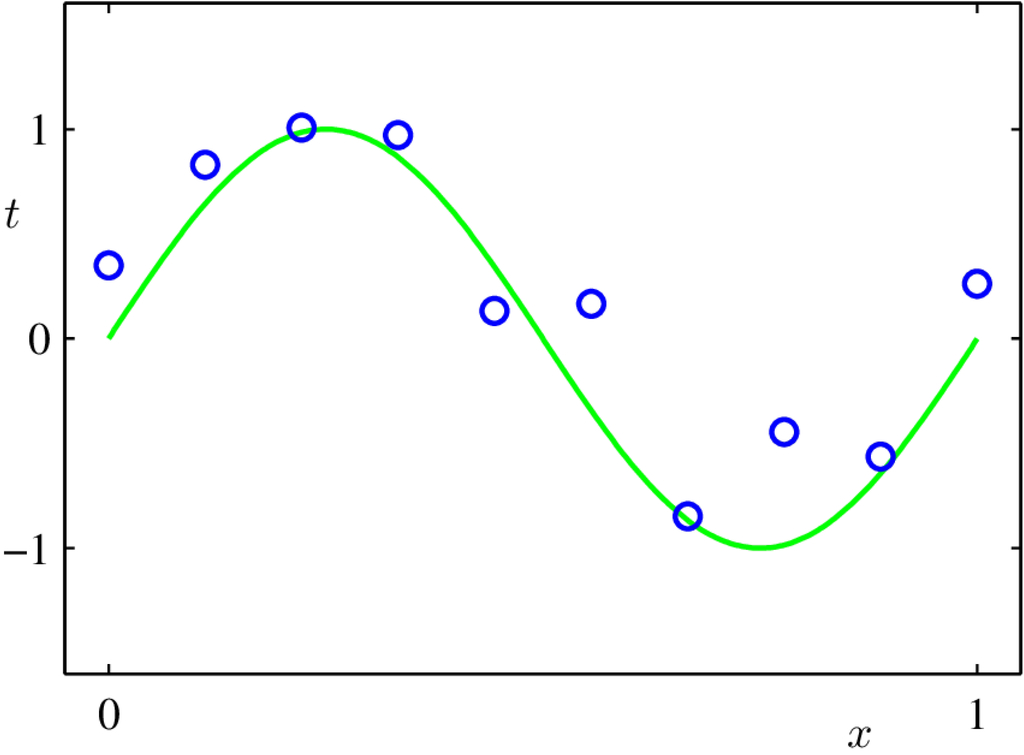
\includegraphics[width=0.61\linewidth]{fig/lec52.jpg}
\end{center}
\end{frame}
% 3
\begin{frame}[c]
\frametitle{Model complexity}
\begin{itemize}
\item Fit a polynomial of order 0
\end{itemize}
\begin{center}
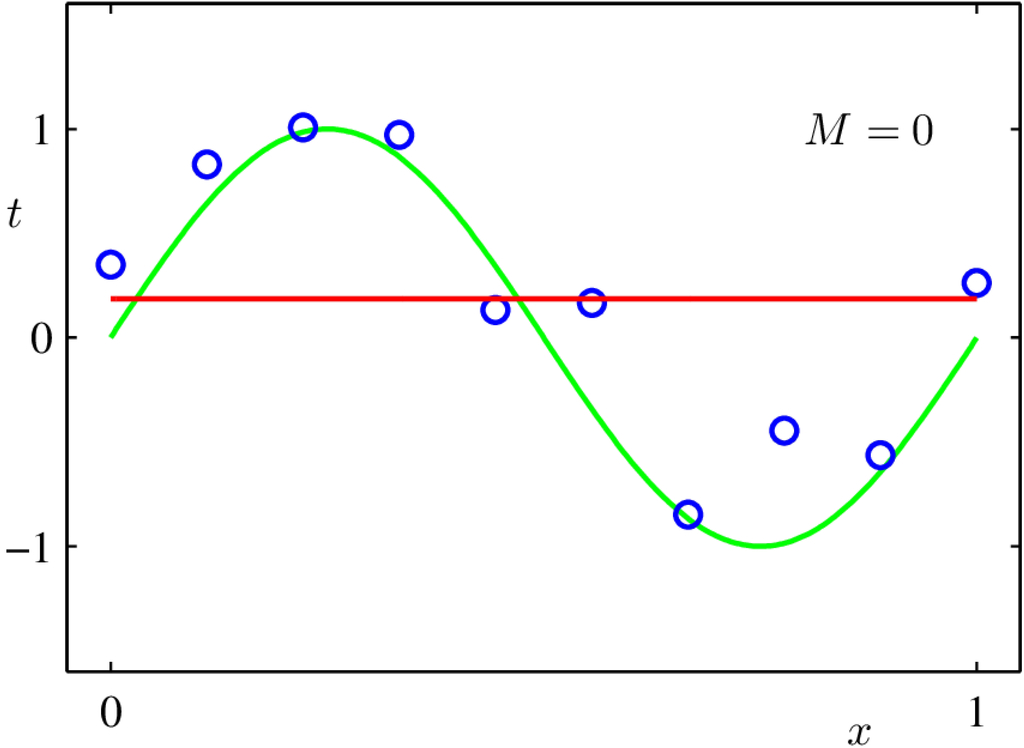
\includegraphics[width=0.61\linewidth]{fig/lec53.jpg}
\end{center}
\end{frame}
% 4
\begin{frame}[c]
\frametitle{Model complexity}
\begin{itemize}
\item Fit a polynomial of order 1
\end{itemize}
\begin{center}
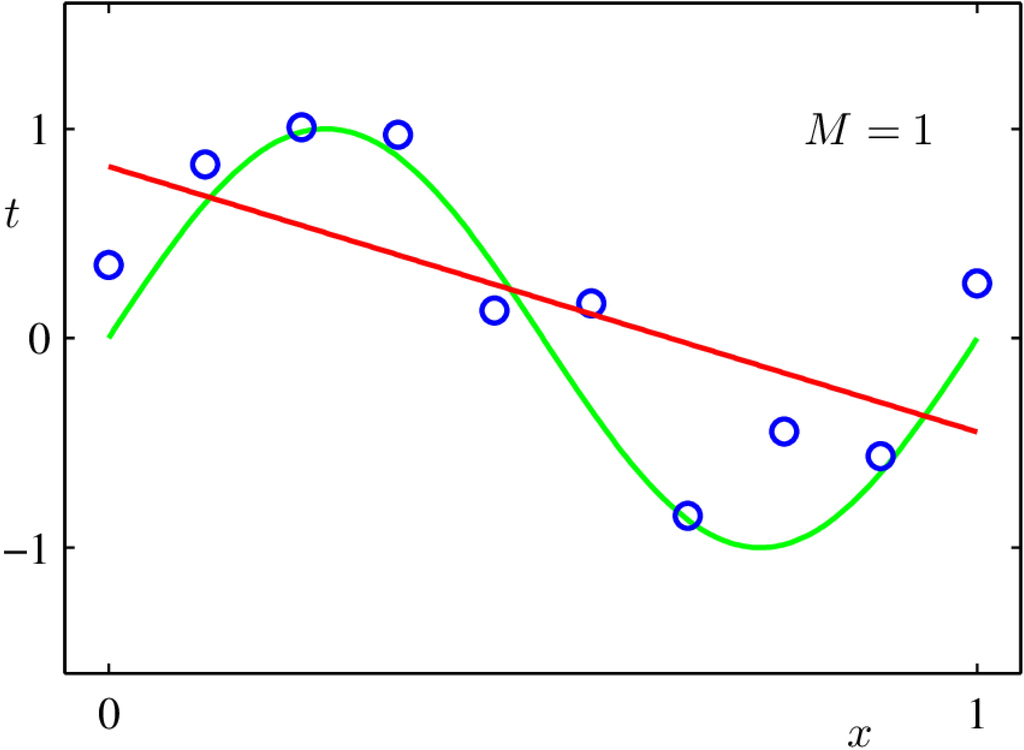
\includegraphics[width=0.61\linewidth]{fig/lec54.jpg}
\end{center}
\end{frame}
% 5
\begin{frame}[c]
\frametitle{Model complexity}
\begin{itemize}
\item Fit a polynomial of order 3
\end{itemize}
\begin{center}
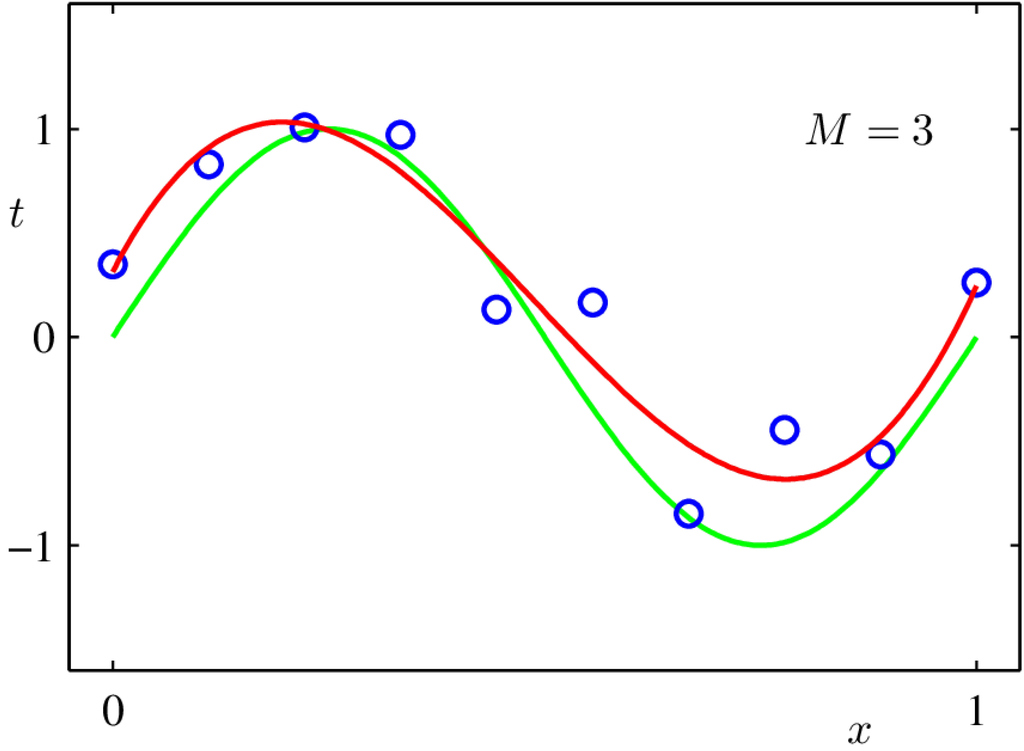
\includegraphics[width=0.61\linewidth]{fig/lec55.jpg}
\end{center}
\end{frame}
% 6
\begin{frame}[c]
\frametitle{\textcolor{black}{Model complexity}}
\begin{itemize}
\item Fit a polynomial of order 9
\end{itemize}
\begin{center}
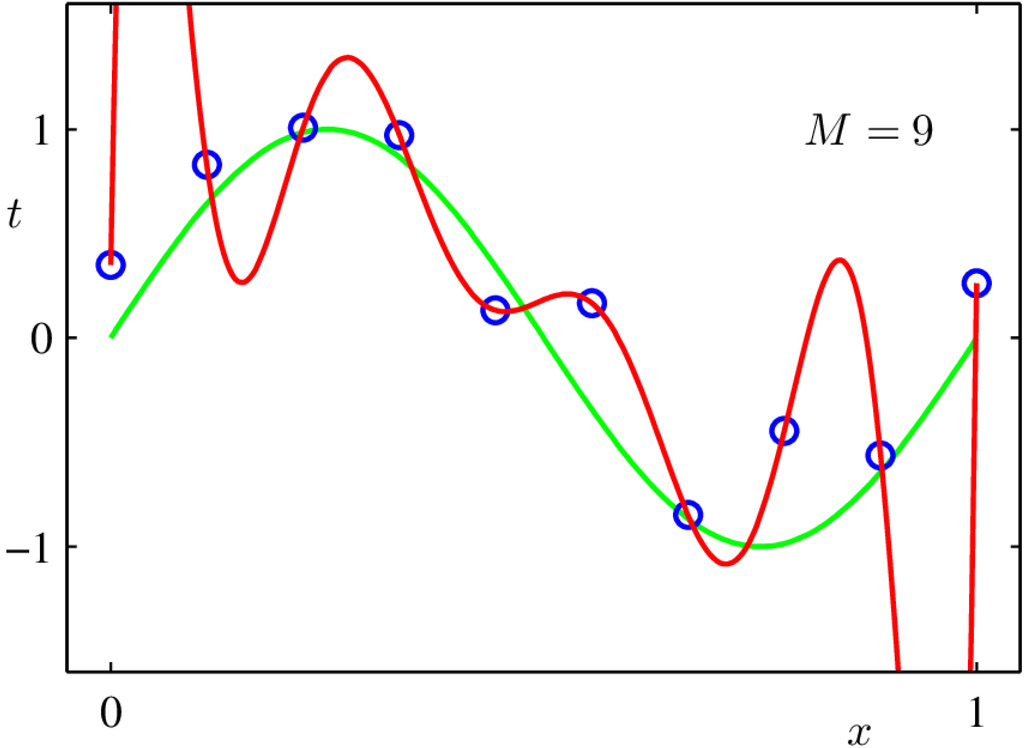
\includegraphics[width=0.61\linewidth]{fig/lec56.jpg}
\end{center}
\end{frame}
% 7
\begin{frame}[c]
\frametitle{Model complexity}
\begin{itemize}
\item Goal of training a machine learning model is {\bf generalization}
		\begin{itemize}
		\item After training on a given set of data
		\item How good will the predictions be on new, unseen data?
		\end{itemize}
\item Create a separate set of data, unseen at training time
		\begin{itemize}
		\item  The test set
		\item Measure performance on it
		\end{itemize}
\end{itemize}
\end{frame}

% 8
\begin{frame}[c]
\frametitle{Model complexity}
\begin{itemize}
\item  Prediction error on training and test sets
\end{itemize}
\begin{center}
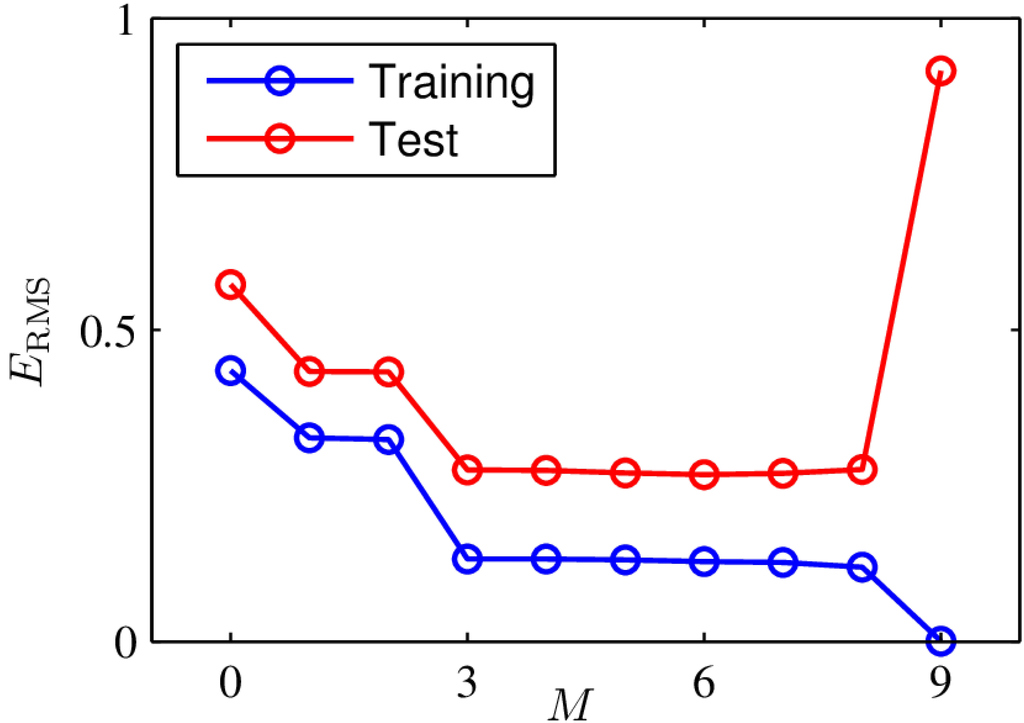
\includegraphics[width=0.61\linewidth]{fig/lec58.jpg}
\end{center}
\end{frame}

% 9
\begin{frame}[c]
\frametitle{Over- vs under-fitting}

\begin{center}
\begin{tabular}{|c|c|c|c|}
\rowcolor{.!30!gray}
&\textcolor{white}{Under-fit}&\textcolor{white}{Good fit}&\textcolor{white}{Over-fit}\\\hline
Training error& High& Low& Low\\\hline
Testing error& High &Low &High\\\hline
\end{tabular}%
\end{center}
\begin{center}
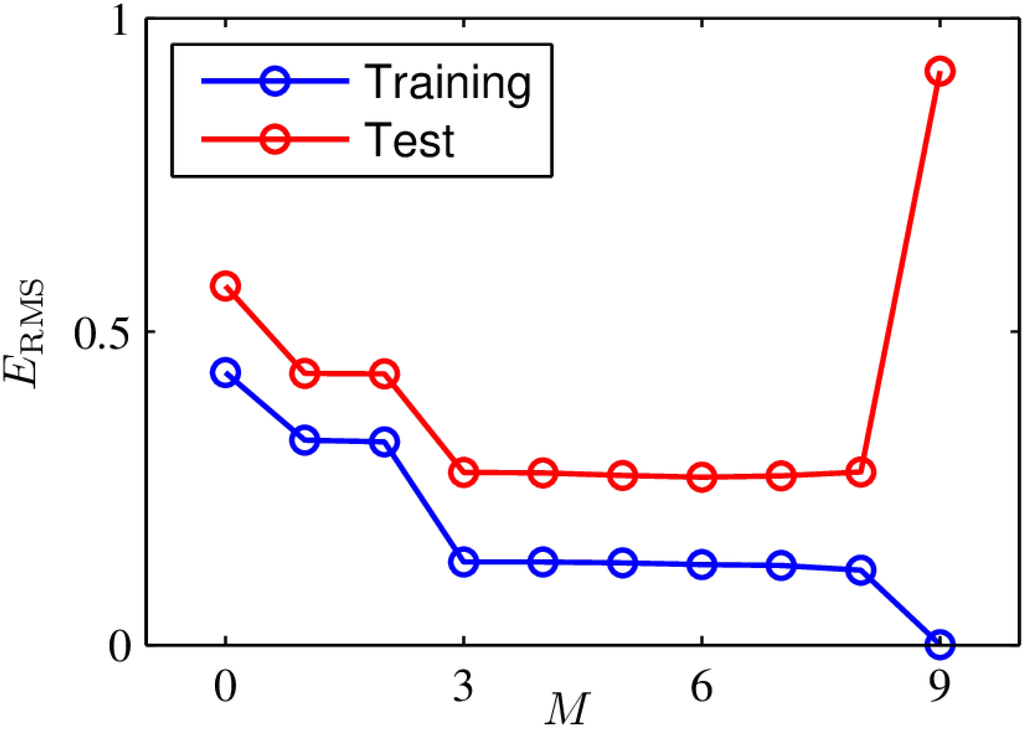
\includegraphics[width=0.61\linewidth]{fig/lec59.jpg}
\end{center}
\end{frame}

% 10
\begin{frame}[c]
\frametitle{Fit depends on amount of data}
\begin{itemize}
\item  Fit a polynomial of order 9, 10 points
\end{itemize}
\begin{center}
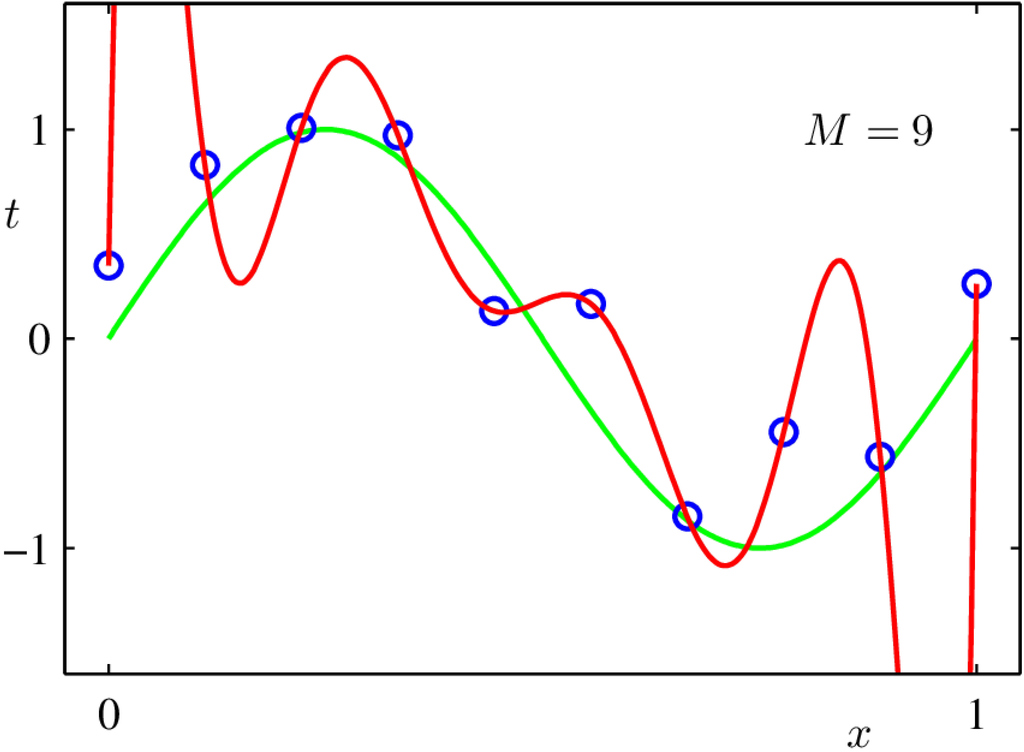
\includegraphics[width=0.61\linewidth]{fig/lec510.jpg}
\end{center}
\end{frame}

% 11
\begin{frame}[c]
\frametitle{Fit depends on amount of data}
\begin{itemize}
\item  Fit a polynomial of order 9, 15 points
\end{itemize}
\begin{center}
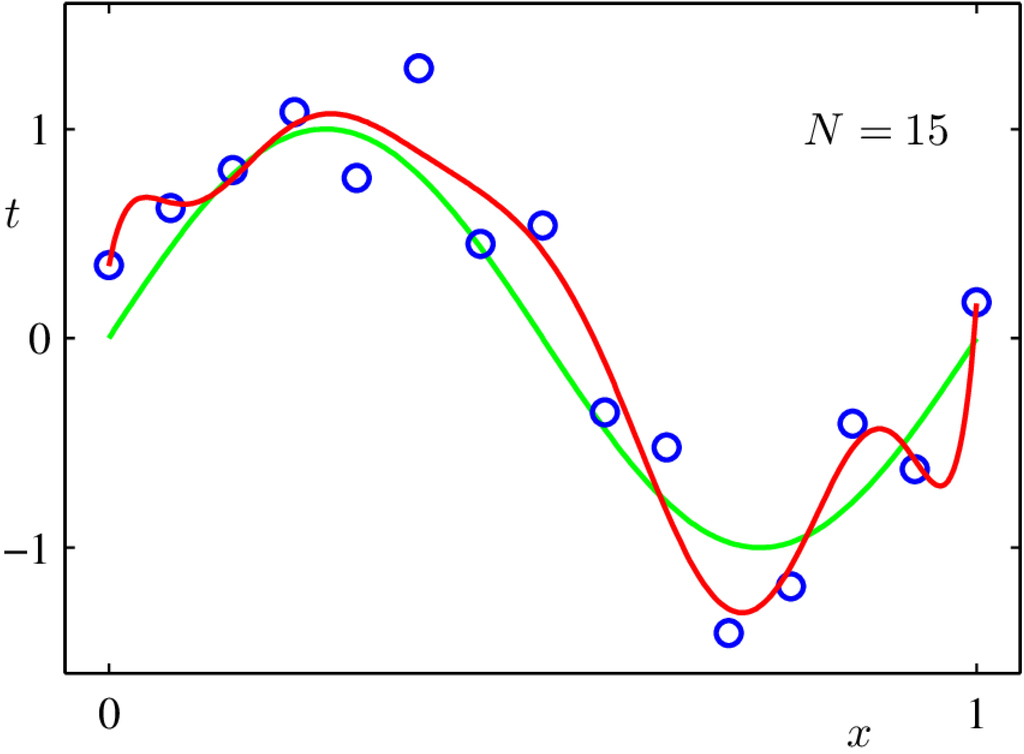
\includegraphics[width=0.61\linewidth]{fig/lec511.jpg}
\end{center}
\end{frame}

% 12
\begin{frame}[c]
\frametitle{Fit depends on amount of data}
\begin{itemize}
\item  Fit a polynomial of order 9, 100 points
\end{itemize}
\begin{center}
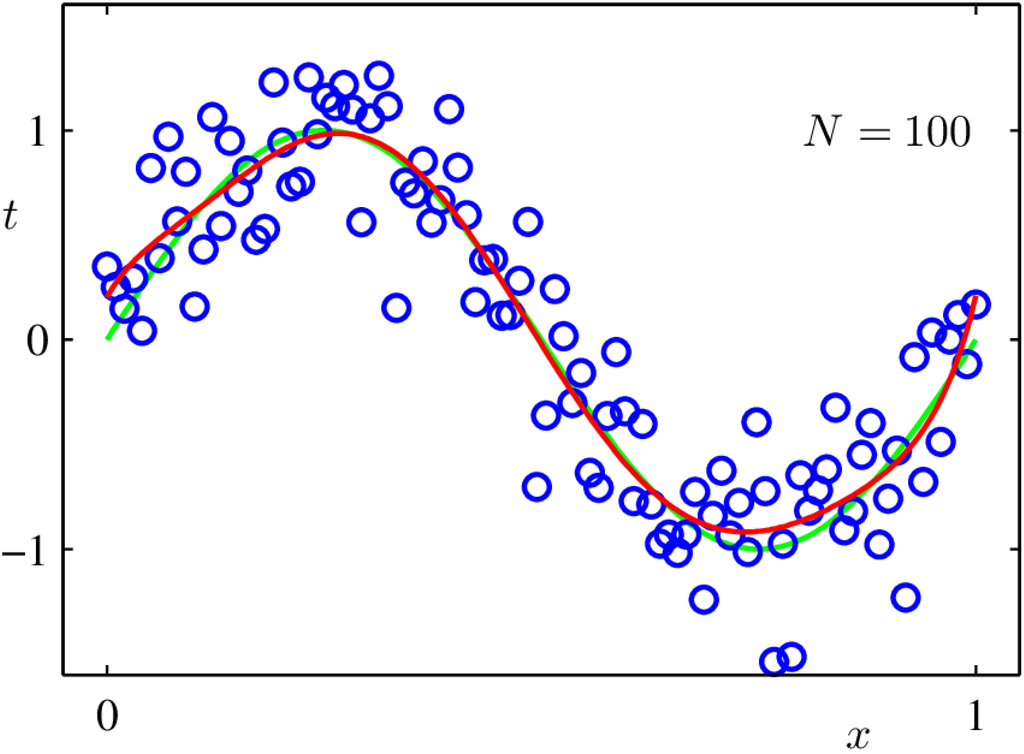
\includegraphics[width=0.61\linewidth]{fig/lec512.jpg}
\end{center}
\end{frame}

% 13
\begin{frame}[c]
\frametitle{Parameter tuning}
\begin{itemize}
\item  What if your model has parameters that need to be tuned?
\item  Need to compare different parameter settings on unseen data
\item  Then need to measure the final selected model on \textit{new} unseen data
\end{itemize}
\end{frame}

% 14
\begin{frame}[c]
\frametitle{Parameter tuning}
\begin{itemize}
\item  3-way division of data: training, validation, and test
		\begin{itemize}
		\item  Train models with different parameters on training set
		\item Measure their performance on validation set
		\end{itemize}
\item  Makes fair comparison of models' abilities to generalize beyond the training set

\item  Select the best-performing model as the final model
		\begin{itemize}
		\item  Measure \textit{only} its performance on the test set
		\item Gives fair estimate of whole system's ability to generalize to new data (i.e., beyond the training and validation sets)
		\end{itemize}
\end{itemize}
\end{frame}


% 15
\begin{frame}[c]
\frametitle{Selecting model parameters: (cross-)validation}
\begin{itemize}
\item  When lots of data is available, use dedicated sets
\item  When data is scarce, use $k$ -fold cross-validation
		\begin{itemize}
		\item  Partition $N$ data points into $k$ sets
		\item Designate one set as the test set
		\item Designate one of the remaining sets as the validation set
		\item Train on the rest, select model on validation
		\item Test on test set
		\item Rotate through the data so that each set is tested on once
		\end{itemize}

\item  Provides unbiased estimate of performance when training on $N~\frac{k-1}{k}$ points and testing on $N$ points
\end{itemize}
\end{frame}

% 16
\begin{frame}[c]
\frametitle{Cross validation illustration}
\begin{center}
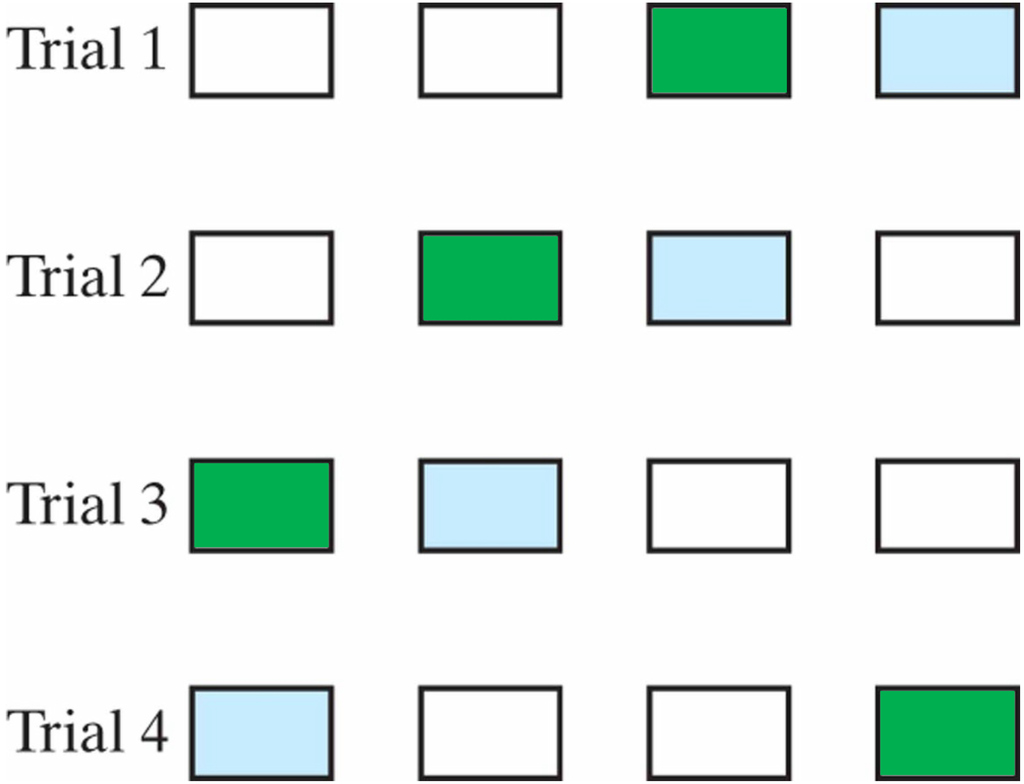
\includegraphics[width=0.61\linewidth]{fig/lec516.jpg}
\end{center}
\end{frame}

% 17
\begin{frame}[c]
\frametitle{Early stopping}
\begin{columns}
\column{.6\textwidth}
\begin{itemize}
\item Now back to MLPs
\item Measure performance on the validation set of models
trained for different numbers of epochs
\item Keep the model with the best validation performance
		\begin{itemize}
		\item And stop training when it looks like a better one isn't coming
		\end{itemize}
\end{itemize}

\column{.3\textwidth}
\begin{center}
\hspace*{-1.3cm}
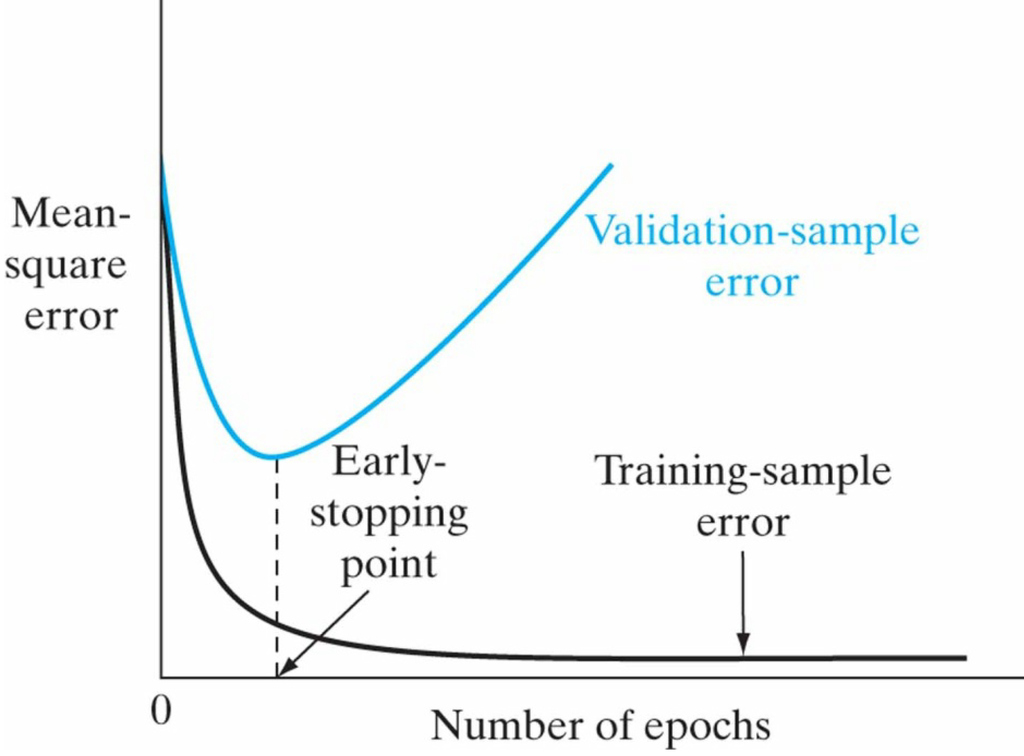
\includegraphics[width=1.6\textwidth]{fig/lec517.jpg}
\end{center}
\end{columns}
\end{frame}









\begin{frame}
\begin{center}
\chuhao Thank you! %\fontspec{LHANDW.TTF}
\end{center}
\end{frame}
\end{document}
